\documentclass[a4paper,oneside,openright,11pt]{book}

\usepackage[T1]{fontenc}

%%%%%%%% Schriftart Latin Modern verwenden:
\usepackage{lmodern}


%%%%%%%% Um Helvetica serifenlos zu verwenden, folgende Zeilen auskommentieren:
%\renewcommand{\familydefault}{\sfdefault}
%\usepackage{helvet} 


\usepackage[utf8]{inputenc} % ggf. Editor auf utf8 stellen!!

\usepackage[ngerman]{babel}

\usepackage{ngerman} % unter anderem für bessere Silbentrennung

\usepackage{listings}
\usepackage{amssymb}
\usepackage{amsmath}
\usepackage{graphicx}
\usepackage{url}
\def\UrlBreaks{\do\/\do-} % Zeilenumbrüche in URLs bei Bindestrich oder Schrägstrich
\usepackage{hyperref}
\usepackage{xspace}
\usepackage{csquotes}


%avoid overfull hbox problem
\setlength{\emergencystretch}{3em}

%avoid underfull hbox problem in bibliography
\usepackage{etoolbox}
% Variant A
\apptocmd{\sloppy}{\hbadness 2000\relax}{}{}
% Variant B
% \apptocmd{\thebibliography}{\raggedright}{}{}

\hyphenpenalty=5000
\tolerance=1000



% standard scaling factor for graphics, to support homogenous looks.
\newcommand{\stdScaleFactor}{0.45}

% Titelseite und Erklaerung
\usepackage{sethesis}


% Angaben Titelseite
\unilogo{
\includegraphics[scale=0.75]{FHDW-Logo.eps}}
%\uniname{}
\fachgebiet{}
\institut{}
\fachbereich{}
% Angaben zur Arbeit
\author{J. Alberts, D. Buchholz, C. Cirak, R. Senemar} % Hier Namen eintragen
\title{Cinema Management Software} % Hier Titel
\englishtitle{}
\ort{Hannover}
\thesistype{Technische Dokumentation}
\studiengang{Informatik} % Hier Studiengang angeben
\erstpru{Prof. Dr. Harald König}
\zweitpru{}
\betreu{}
\datum{\today} % Datum der Abgabe hier einsetzen

% Sonstiges
%\allowdisplaybreaks
%\setlength{\parindent}{1em}
%\setlength{\parskip}{0em}
%\makeatletter
%\renewcommand{\fps@figure}{ht!}
%\renewcommand{\fps@table}{ht!}
%\setlength{\@fptop}{0pt}
%\makeatother


\begin{document}

\frontmatter

\maketitle

\clearpage
\chapter*{Zusammenfassung}

Kurze Zusammenfassung der Arbeit in ca. 200 Wörtern

\clearpage

\chapter*{Abstract}

An optional summary of approx. 200 words.


\clearpage



\tableofcontents

\mainmatter

\chapter{Einleitung}
\label{chap:einleitung}

In diesem Dokument beschreiben wir die  formale Anforderungen an die Prüfungsmodule
\begin{itemize}
    \item Praxisarbeit (1. und 2. Praxisarbeit im Bachelor)
    \item Bachelor-Thesis
    \item Lehrprojekt (Master)
    \item Master-Thesis
\end{itemize}
in den \textbf{technischen Studiengängen der FHDW Hannover}.
Dieses Dokument ist auch Richtlinie für das Anfertigen von Berichten für Transferprojekte im technischen Bereich (als Teil eines Aufbaustudiums). 

Zunächst beschreiben wir formale Anforderungen in Kapitel~\ref{chap:anforderungen}. Kapitel~\ref{chap:struktur-und-inhalt} beschreibt Unterschiede zwischen den oben genannten Prüfungsformen und Anforderungen an deren Inhalt und Struktur, die sich daraus ergeben. In Kapitel~\ref{chap:bewertungskriterien} beschreiben wir Bewertungskriterien, die wir bei der Bewertung der Arbeiten zugrundelegen.

Zudem ist dieses Dokument mit Hilfe einer \textbf{\LaTeX{}-Vorlage} geschrieben, die wir Ihnen als Vorlage für das Verfassen Ihrer Arbeiten empfehlen.

Diese Vorlage erhalten Sie hier:

\begin{center}
    \url{https://www.overleaf.com/read/yrndghycwxgb}
\end{center}





\chapter{Formale Anforderungen}
\label{chap:anforderungen}

\section{Allgemeiner Hinweis}

Die Erstellung von Abschlussarbeiten und Projektarbeiten unterliegt bestimmten formalen Regelungen. 
Im Folgenden unterscheiden wir zwischen

\begin{itemize}
    \item \textbf{Verbindlichen Vorschriften}, die für die Erstellung von wissenschaftlichen Arbeiten an der FHDW Hannover unbedingt einzuhalten sind und
    \item \textbf{Empfehlungen}, zu weiteren Aspekten, bei denen ein Gestaltungsspielraum besteht. Diesen sollten Sie folgen und mit dem jeweiligen Betreuer abstimmen.
\end{itemize}

\section{Welches Textverarbeitungsprogramm?}

Sie können das Textverarbeitungsprogramm wählen. Wir empfehlen Ihnen die Verwendung von \LaTeX{} und insbesondere die Verwendung dieser Vorlage:

\begin{center}
 \url{https://www.overleaf.com/read/yrndghycwxgb}   
\end{center}

Zudem können wir die Verwendung des Online-Editors Overleaf (\url{https://www.overleaf.com/}) empfehlen. Haben Sie keine stabile Internetverbindung oder verstößt die Verwendung von Online-Editoren gegen Geheimhaltungsrichtlinien, nutzen Sie Offline-Editoren wie zum Beispiel TexStudio (\url{https://www.texstudio.org/}). Recherchieren Sie online nach Installationshinweisen.

Es gibt im Internet viele gute Quellen für den Einstieg in \LaTeX{}, zum Beispiel \url{https://www.overleaf.com/learn/latex/Learn_LaTeX_in_30_minutes}. Recherchieren Sie selbst weitere Quellen!

\LaTeX{} bietet viele Vorteile, zum Beispiel beim Umgang mit Referenzen, Quellverweisen oder mathematischen Formeln. Auch ist die typographische Qualität in von \LaTeX{} generierten Dokumenten meist besser als in mit Word geschriebenen Dokumenten (\url{https://openwetware.org/wiki/Word_vs._LaTeX}). In fast allen naturwissenschaftlichen Bereichen werden Veröffentlichungen heute mit \LaTeX{} verfasst. \LaTeX{} erfordert ein wenig Einarbeitungsaufwand, aber die Investition darin lohnt sich! Sie werden es nicht bereuen!

Unabhängig von der Wahl des Textverarbeitungsprogramms empfehlen wir Ihnen dringend, in regelmäßigen Abständen Sicherungskopien Ihrer Arbeit anzulegen, sodass Systemabstürze oder ein Verlust des Laptops nicht zu Problemen bei der fristgerechten Abgabe der Arbeit führen.

\section{Umfang der Arbeit}

In Tabelle~\ref{tab:seitenumfang} sind die erlaubten Seitenumfänge für die einzelnen Prüfungsleistungen aufgelistet.
Die Seitenumfänge beziehen sich auf die Seiten des \textit{Inhaltsteils} der Arbeit (s. auch Abschnitt~\ref{sec:bestandteile-der-arbeit}); Titelblatt, Erklärungen, Verzeichnisse und Anhang zählen also nicht mit.

\begin{table}[ht]
\centering
\begin{tabular}{|p{8cm}| p{3cm}|}
\hline
     1. und 2. Praxisprojekt (Bachelor) & 20 bis 22 Seiten \\\hline
     Bachelor Thesis & 40 bis 44 Seiten \\\hline
     Lehrprojekt (Master) & 30 bis 33 Seiten \\\hline
     Master Thesis & 60 bis 66 Seiten \\\hline
     Transferprojekt (Praxisprojekt Aufbaustudium) & 25 bis 30 Seiten \\\hline
\end{tabular}
\caption{\label{tab:seitenumfang}Vorgeschriebene Seitenumfänge.}
\end{table}

In Absprache mit dem Erstprüfer können Sie im Ausnahmefall eine abweichende Seitenzahl vereinbaren.


\section{Bestandteile der Arbeit}
\label{sec:bestandteile-der-arbeit}

Die Arbeit hat grundsätzlich folgende Bestandteile in folgender Reihenfolge:

\begin{enumerate}
    \item Titelblatt mit Namen, Nachnamen, Studiengang, Namen des Prüfers (Praxisarbeit und Lehrprojekt) oder der Prüfer (Erst- und Zweitprüfer bei Bachelor- und Master-Thesis), sowie Abgabedatum
    \item Eine ehrenwörtliche Erklärung (Hier müssen Sie den genauen Wortlaut des Textes in dieser Vorlage übernehmen, siehe Seite~\pageref{chap:erklaerung-selbstaendigkeit})
    \item \textit{Optional:} Eine Geheimhaltungserklärung oder Sperrvermerk (dieses Template enthält eine Vorlage, siehe \texttt{restriction-notice.tex}, welche Sie im Hauptdokument einbinden können, siehe \texttt{meinearbeit.tex})
    \item \textit{Optional:} Eine kurze Zusammenfassung der Arbeit (maximal eine Seite), optional auch in englischer Version (Abstract).
    \item  \textit{Optional:} Einen Glossar
    \item Ein Inhaltsverzeichnis mit Seitenangaben
    \item Einen Inhaltsteil inklusive Abbildungen und Tabellen
    \item Ein Quellverzeichnis
    \item \textit{Optional:} Ein Abbildungs- und/oder Tabellenverzeichnis
    \item \textit{Optional:} Einen Anhang
\end{enumerate}

\section{Seitenzahlen}

Die Seitenzählung mit arabischen Zahlen beginnt auf der ersten Seite des Inhaltsteils und erfolgt so fortlaufend bis zum Arbeitsende inklusive Quellverzeichnis und Anhang. Die Seiten am Anfang der Arbeit vor der ersten Inhaltsseite, also die Seiten mit der ehrenwörtlichen Erklärung und dem Inhaltsverzeichnis, nummerieren Sie mit kleinen römischen Zahlen (i, ii, iii, iv, ...).

\section{Schriftart}

Verwenden Sie gängige und gut lesbare Schriftarten in Schriftgröße 11pt. Verwenden Sie keine \enquote{Narrow}-Schriftarten. Viele empfinden, dass Serifen-Schriften für Fließtext besser lesbar sind. Sie können aber auch serifenlose Schriften verwenden. 

\paragraph{\textit{Empfehlungen}:}

\begin{itemize}
    \item In \LaTeX{} verwenden Sie Latin Modern oder Helvetica. Im Hauptdokument dieser Vorlage finden Sie Instruktionen für die Einstellung der Schriftart. Nutzen Sie ein anderes Textverarbeitungsprogramm, verwenden Sie Times New Roman, Garamond, Arial oder ähnliche Schriftarten.
    \item Wenn Sie neue Begriffe definieren oder erklären, verwenden Sie dabei den \textit{Kursivdruck}.
    \item Wichtige Schlagworte im Text können \textbf{fett} hervorgehoben werden. Aber: setzen Sie dieses Stilmittel nur sparsam ein!
\end{itemize}




\section{Kapitel, Abschnitte und Nummerierung}

Der Inhalt der Arbeit muss in Kapitel und Abschnitte strukturiert sein. Abschnitte können Unterabschnitte enthalten. Nummerieren Sie Kapitel, Abschnitte und Unterabschnitte nach dem Dezimalsystem (1, 1.1, 1.1.1 etc.). Im Inhaltsverzeichnis werden die niedrigeren Gliederungsebenen eingerückt.

Nummerieren Sie auch Abbildungen und Tabellen im Dezimalsystem, zum Beispiel Abbildung~1, Tabelle~1. Sie können auch die Kapitelnummer mit den Abbildungs- und Tabellennummern kombinieren, zum Beispiel Abbildung~1.1, Tabelle~1.1 -- wie in dieser Vorlage. Dasselbe gilt für Tabellen und Listings von Quellcode. Bedenken Sie: Abbildungen haben \textit{Unterschriften}, Tabellen und Listings hingegen haben \textit{Überschriften}.

Für Verweise auf Abschnitte, Abbildungen, Quellcode oder anderweitige Verweistypen verwenden Sie die automatischen Mechanismen des Textverarbeitungsprogramms. In \LaTeX{} verwenden Sie Label und Referenzen darauf.

\paragraph{\textit{Empfehlungen}:}

Die Überschriften der einzelnen Gliederungspunkte sollten möglichst aussagekräftig sein. Dasselbe gilt für die Beschriftungen von Abbildungen und Tabellen. Der Text in den Abschnitten sollte in Absätze unterteilt sein. Merksatz: \enquote{Pro Satz ein Gedanke, pro Absatz ein Gedankengang}. Ein Absatzbeginn kann, wie in dieser Vorlage, eingerückt sein, wobei es nach Überschriften keine Einrückungen geben sollte.


\section{Seitenformat und Ränder}

Die Arbeit muss im Seitenformat A4 formatiert sein. Sie können ein ein- oder zweiseitiges Format wählen. Ein zweiseitiges Format ist sinnvoll, wenn Sie die Arbeit auf Papier drucken und binden möchten. Sonst ist eine einseitiges Format besser geeignet. Den Text setzen Sie in Blocksatz.

Nutzen Sie folgende Einstellungen für Ränder:
\begin{itemize}
    \item \textit{einseitiges} Dokument: links: 3-4cm, rechts: 4-5cm, oben und unten: 4-5cm
\end{itemize}

Wenn Sie diese \LaTeX{}-Vorlage verwenden, verändern Sie \textbf{nicht} die Einstellungen der Ränder.

\section{Sprache}

Im Regelfall sollten Sie die Arbeit auf Deutsch verfassen. Sie können auch auf Englisch schreiben. Besprechen Sie das vorher mit Ihrem Erstprüfer.

\paragraph{\textit{Empfehlung}:}
Schreiben Sie in einem Textverarbeitungsprogramm wie Word oder LibreOffice Writer, sollten Sie die Funktion \enquote{Automatische Silbentrennung} nutzen, um größere Lücken im Text (Blocksatz) zu vermeiden. Schreiben Sie in \LaTeX{}, stellen Sie sicher, dass die richtige Sprache für die Silbentrennung konfiguriert ist und fügen Sie bei Bedarf benutzerdefinierte Trennregeln hinzu (siehe zum Beispiel \url{https://www.overleaf.com/learn/latex/German}).

\section{Abbildungen}

Wo sinnvoll, sollte Ihre Arbeit Grafiken und Schaubilder enthalten. Fügen Sie diese wenn möglich in einem \textbf{Vektorformat} ein. Bitmap-Formate wie JPG oder PNG sollten nur in Ausnahmen verwendet werden.

Abbildung~\ref{fig:feature-diagram-productioncell-example} ist ein Beispiel für das Einbinden einer Grafik. In \LaTeX{} können Sie Vektorgrafiken in Form von PDF oder EPS einbinden. Die meisten Zeichen- und Modellierungswerkzeuge unterstützen den Export von PDFs.

\begin{figure}[h]
 \centering
 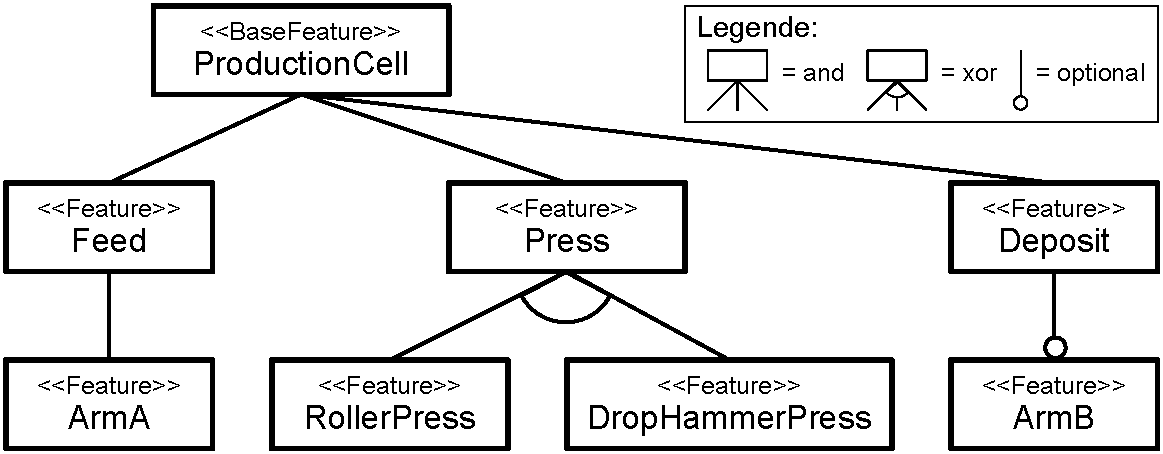
\includegraphics[scale=\stdScaleFactor]
 {contents/figures/feature-diagram-productioncell-example.pdf}
 \caption{Das Featurediagramm eines Produktionsroboters}
 \label{fig:feature-diagram-productioncell-example}
\end{figure}

Achten Sie darauf, dass jede ung gut lesbar ist und nicht den Rand des Textbereichs überschreitet. Eine Abbildung muss immer im Text referenziert und beschrieben werden. Was sieht der Leser? Was bedeuten zum Beispiel verschiedene Pfeile? Eine Legende in der Grafik (wie in Abb.\,\ref{fig:feature-diagram-productioncell-example}) ist nicht zwingend notwendig, kann die Grafik aber besser verständlich machen. Sie können das Wort "`Abbildung"' im Text mit "`Abb."' abkürzen. An Satzanfängen sieht die ausgeschriebene Variante allerdings schöner aus.

\paragraph{\textit{Empfehlungen}:}

\begin{itemize}
    \item Positionieren Sie Abbildungen möglichst nah an der Stelle, wo sie im Text referenziert und erklärt werden. In \LaTeX{} benutzen Sie für das Einbinden von Abbildungen mittels der \texttt{figure}-Umgebung am besten den Parameter \texttt{[h]}: 
    
    \begin{verbatim}
        \begin{figure}[h] ... \end{figure}
    \end{verbatim}
    
    \item In Abbildungen nutzen Sie besser serifenlose Schriften, wie zum Beispiel Arial. Die Schrift in Grafiken sollte etwas kleiner als der Fließtext sein, ca. 60\%-90\%, aber nicht weniger als 50\%, da die Schrift sonst zu klein und nicht mehr lesbar wird. Außerdem sollten die Schriften in Abbildungen konsistent in der Größe sein. Verwenden Sie daher eine einheitliche Schrift und Schriftgröße in den Abbildungen und einen einheitlichen Skalierungsfaktor für Abbildungen im Text.
\end{itemize}



\section{Schreibstil}

\subsection{Aktiv und Passiv, Verwendung von \textit{ich}}

Der wissenschaftliche Schreibstil hat sich in den letzten Jahren gewandelt. Früher waren lange, verschachtelte Sätzen ein Zeichen von Wissenschaftlichkeit und Autoren schrieben in passiver Form, um die Personalpronomen \enquote{wir} und \enquote{ich} zu vermeiden -- \enquote{wir} und \enquote{ich} klinge \enquote{weniger objektiv}, so oft die Begründung.

Das hat sich geändert. Heute ist es in technischen Bereichen, auch durch den angelsächsischen Einfluss, ein Zeichen guten Ausdrucks, möglichst im Aktiv zu schreiben. Passive Sätze wirken distanziert und sind oft komplizierter als aktive Sätze. Daher raten wir zur aktiven Sprache. 

Wenn Sie in der Arbeit Ihr eigenes Vorgehen, Abwägungen oder Entscheidungen beschreiben, sollten Sie insbesondere die Personalpronomen \enquote{wir} und \enquote{ich} verwenden. Diese Ausführungen sind inhärent \textit{subjektiv} und sollten auch nicht den falschen Anschein von Objektivität erwecken.

In wissenschaftlichen Veröffentlichungen im technischen Bereich wird oft \enquote{wir} (oder engl. \enquote{we}) verwendet, ein \enquote{ich} findet man seltener. Das liegt allerdings daran, dass wissenschaftliche Arbeiten meist von mehr als einer Person durchgeführt und veröffentlicht werden. Selbst wenn eine Veröffentlichung nur einen Autor hat, schreibt dieser Autor meist \enquote{wir}, weil die Arbeit selten von dem Autor allein stammt, sondern auch eine Forschergruppe dahinter steht.

Bei studentischen Arbeiten ist das anders, da diese eigenständige Studienleistungen sind, die Sie auch wirklich allein bearbeiten müssen. Zudem müssen Sie in der schriftlichen Darstellung deutlich machen, welche Ergebnisse Sie persönlich produziert haben und welche Beiträge anderen zuzuschreiben sind, zum Beispiel Kollegen im Partnerunternehmen.

Nehmen wir den passiven Satz \enquote{Es wurde eine Problemanalyse durchgeführt und Anforderungen wurden abgeleitet.} -- Wer hat denn die Problemanalyse durchgeführt und Anforderungen abgeleitet? Der Autor des Textes? Oder bezieht sich der Autor auf Vorarbeiten von Kollegen? Das wird in dieser Formulierung nicht klar! 

Schreiben Sie besser \enquote{Ich habe eine Problemanalyse durchgeführt und Anforderungen abgeleitet}. Haben vielleicht Kollegen dabei geholfen? Welchen Anteil hatte dabei der Kollege? Machen Sie dies explizit deutlich und schreiben Sie zum Beispiel: \enquote{Ich habe eine Problemanalyse durchgeführt und eine erste Liste von Anforderungen abgeleitet. Diese Liste habe ich daraufhin zusammen mit Kollegen der Abteilung konkretisiert und priorisiert.} Nun wird deutlich, welchen Beitrag Sie geleistet haben! Ihre Prüfer können Ihre Leistung nun eindeutiger beurteilen.

Gehen Sie jedoch sparsam mit \enquote{ich} oder \enquote{wir} um und beschränken Sie deren Verwendung auf Stellen, an denen Sie Ihr eigenes Vorgehen, Abwägungen oder Entscheidungen beschreiben -- eine Praxis- oder Abschlussarbeit ist kein Tagebuch und keine Erzählung aus der Ich-Perspektive!

Die passive Schreibweise müssen Sie natürlich nicht vollständig verbannen. Dort wo eine Handlung im Vordergrund steht und nicht der Handelnde, können Sie das Passiv verwenden. Beispiel: \enquote{Bei der testgetriebenen Entwicklung werden Anforderungen bereits in Testfälle überführt, bevor die entsprechende Softwarefunktionen entwickelt werden.} Jedoch kann es auch hier hilfreich sein, zu erklären, welche Personen oder Rollen am Geschehen beteiligt sind -- gerade wenn es um Arbeitsprozesse geht. Wer schreibt die Tests? Ein Tester? Der Entwickler selbst? Vielleicht ist es doch besser zu schreiben \enquote{Bei der testgetriebenen Entwicklung überführt der Entwickler oder die Entwicklerin die Anforderungen in Testfälle, schon bevor er/sie die entsprechenden Softwarefunktionen entwickelt.}

\subsection{Wortwahl}

Vermeiden Sie lange, verschachtelte Sätze sowie überflüssige Worte und vage Formulierungen.

\paragraph{\textit{Empfehlung}:}
Es gibt viele Quellen, auch online, mit Tipps zum Schreiben. Recherchieren Sie und reflektieren Sie über Ihre Ausdrucksweise.


\section{Arbeit mit Quellen}
\label{sec:arbeit-mit-quellen}

Bei der Erklärung von Grundlagen, Problemstellungen, Lösungsansätzen, verwandten Arbeiten oder zur Unterstützung von Argumenten sollten Sie auf geeignete Quellen hinweisen. Hier Beispiele für Referenzen auf Quellen~\cite{Greenyer2007,Greenyer2013}, welche im Quellverzeichnis aufgelistet sind. 
Sie können numerische oder auch alphabetische Verweisstile verwenden (siehe auch \url{https://www.overleaf.com/learn/latex/Articles/Getting_started_with_BibLaTeX}). Verwenden Sie für Zitate keine Fußnoten, wie dies in anderen Bereichen üblich ist.

Achten Sie beim Quellenverzeichnis darauf, dass dort alle Quellen aufgelistet sind, die Sie im Text zitiert haben (und auch nur diese!).

\paragraph{\textit{Empfehlung}:}
Wenn Sie mit \LaTeX{} arbeiten, verwenden Sie \textit{Bibtex}. Für mehrere Quellverzeichnisse verwenden Sie \textit{Multibib} (\url{https://www.overleaf.com/learn/latex/Multibib}).

Sie können die Quellen in ein Quellverzeichnis sortieren oder mehrere Quellverzeichnisse nach Publikationstyp getrennt verwenden. Dieses bietet sich an um wissenschaftliche Quellen und nicht-wissenschaftliche Quellen eindeutig zu trennen, ist aber optional.

\subsection{Korrekt zitieren}

Achten Sie auf die Vollständigkeit der Quellenangaben. Wenn Sie \LaTeX{} und Bibtex verwenden, werden die Angaben meist automatisch in der richtigen Reihenfolge generiert. Sie können oft auf den Webseiten der Verlage fertige Bibtex-Einträgen zu Quellen finden. Viele Verlage, wie zum Beispiel Springer, ACM, IEEE, etc. (s. Links unten), bieten für ihre Veröffentlichungen meist vollständige und korrekte Bibtex-Einträge zum Download an. Zur Verwaltung von Quellen können Sie Werkzeuge wie JabRef (\url{https://www.jabref.org/}) nutzen, welches auch Funktionen für die Suche und den automatischen Import von Bibtex-Einträgen bietet. Wenn Sie irgendwo anders im Internet Bibtex-Einträgen finden, vertrauen Sie nicht darauf, dass diese vollständig und richtig sind. Prüfen Sie in jedem Fall die finale Darstellung Ihre Quellenangaben im Dokument. 

Erforderliche Angaben zu den Quellen, je nach Art der Quelle, sind im Folgenden beschrieben:

\begin{itemize}
    
    \item \textbf{Monographien und Lehrbücher} (Bibtex-Typ \texttt{@book}): 
    Es erscheinen zuerst die Autoren mit erst Nachname, dann Vorname. Es folgt ein Punkt oder Doppelpunkt (aber: konsistent bleiben), dann der Titel der Publikation, Verlag und optional Erscheinungsort(e). Danach folgt die Zahl der Ausgabe, falls nicht die erste. Zuletzt wird das Jahr der Veröffentlichung genannt. Beispiel: \cite{Sutton2018}
    
    \item \textbf{Fachartikel in Zeitschriften} (Bibtex-Typ \texttt{@article}): 
    Wieder erscheinen zuerst die Autoren, dann der Titel des Artikels. Es folgt der Zeitschriftentitel sowie die Heftnummer (number),  Band (volume), Seitenbereich und Jahresangabe. Beispiel: \cite{Greenyer2013}
    
    \item \textbf{Konferenzbeiträge} (Bibtex-Typ \texttt{@inproceedings}): 
    Wieder erscheinen zuerst die Autoren, dann der Titel des Artikels. Es folgt die Nennung des Konferenzbandes, wobei, wenn bekannt, die Herausgeber (Editoren) des Konferenzbandes vorangestellt werden.
    Darauf folgt optional Serie, Heftnummer und Band, und schließlich Seitenbereich und Jahresangabe. Beispiel: \cite{Greenyer2007}
    
    \item \textbf{Internetquellen} (Bibtex-Typ \texttt{@misc}): Sie können auch Online-Artikel, Wikipedia-Einträge, API-Referenzen, Podcasts, Blog-Einträge, Videos, Social-Media-Beiträge oder andere Quellen im Internet zitieren.
    Geben Sie auch hier erst, soweit vorhanden, die Namen der Autoren an, dann den Titel, gegebenenfalls den Namen eines Online-Magazins, ein Veröffentlichungsdatum, dann die URL der Quelle und das Zugriffsdatum. Beispiel: \cite{Gebhard2021}
    
    \item Es gibt weitere Arten von Quellen, wie Buchkapitel, Masterarbeiten, Doktorarbeiten, technische Berichte oder Standards. Auch hier werden zuerst Autoren und dann der Titel genannt. Weiter Angaben variieren. Recherchieren Sie nach einer gängigen Zitierweise und korrekter Nutzung von Eintrags-Typen in Bibtex. Hier ein Beispiel für den Verweis auf einen Standard: \cite{UML251}.
\end{itemize}


\subsection{Zitate im Text}

Wenn Sie Textstellen wörtlich oder wörtlich übersetzt aus anderen Quellen wiedergeben, müssen Sie diese Textbereiche \textbf{eindeutig durch Anführungszeichen} kennzeichnen.
Hier ein Beispiel für ein wörtliches, übersetztes Zitat: \enquote{Heute werden oft nicht nur einzelne Softwareprodukte entwickelt, sondern ganze Produktlinien, also es müssen viele Varianten eines Produkts entwickelt werden.} \cite[Seite~1]{Greenyer2013}.

\textbf{\textit{Empfehlung:}} Gehen Sie sparsam mit übernommenen Textpassagen um. Wörtlich übernommene Textpassagen sollen Ihre eigenen Inhalte ergänzen und unterstützen, diese nicht ersetzen. Wenn ein Grundlagen-Kapitel eine Aneinanderreihung kopierter Passagen aus fremden Quellen ist, werden die Inhalte nicht als Ihre kreative Leistung anerkannt.

Allgemein sollte eine Referenz nicht als Textelement genutzt werden\footnote{Dasselbe gilt für Fußnoten. Fußnoten sollten übrigens nur in Ausnahmefällen eingesetzt werden, wenn eine zusätzliche Anmerkung nur sehr schwer im Haupttext erwähnt werden kann, ohne den Textfluss, wie zum Beispiel eine Argumentationskette, zu unterbrechen. Eine gute Arbeit kommt sehr gut ohne Fußnoten aus: Sind Anmerkungen wichtig, sollten sie in den Haupttext integriert werden. Sind sie nicht wichtig, warum sollten sie dann in der Arbeit erwähnt werden? Oder fanden Sie es jetzt gut, vom Lesefluss abgelenkt zu werden, nur um hier etwas im Kleingedruckten zu lesen und gleich wieder die Textstellen suchen zu müssen, wo Sie weiterlesen wollten?}. Also nicht so: Eine effiziente Methode zur Konsistenzanalyse wird in~\cite{Cordy2012} beschrieben. Sondern so: Eine effiziente Methode zur Konsistenzanalyse wird beschrieben von Cordy et al.\,\cite{Cordy2012}. Der Text sollte also auch lesbar sein, wenn die Verweise entfernt würden. Die Abkürzung \textit{et al.} bedeutet übrigens \enquote{et alii}, auf Deutsch \enquote{und andere}; diese Ausdruck wird in wissenschaftlichen Schriften gerne verwenden, wenn von mehr als zwei Autoren die Rede ist, um diese nicht alle aufzählen zu müssen.

Wenn Sie zitieren, sollten sie, zumindest in einer Bachelor- oder Master-Thesis, möglichst wissenschaftliche Quellen zitieren. Das sind Papiere von Workshops und Konferenzen, sowie Dissertationen, Fachbücher oder Artikel in Fachjournalen. Diese Quellen sind meist vertrauenswürdig, da sie einen Begutachtungsprozess durchlaufen. Technische Berichte werden typischerweise nicht begutachtet, sind aber meist vertrauenswürdig wenn Sie von Wissenschaftlern verfasst sind, die weitere, begutachtete Papiere zu demselben Themenbereich veröffentlicht haben.

Bei der Recherche sind diese Internetseiten hilfreich:
\begin{itemize}
  \item \url{http://scholar.google.com}
  \item \url{http://academic.research.microsoft.com/}
  \item \url{http://ieeexplore.ieee.org/}
  \item \url{http://dl.acm.org/dl.cfm}
  \item \url{http://www.springerlink.com/}
  \item \url{https://www.springerprofessional.de/} (die FHDW hat hier Zugänge -- sprechen Sie Ihren Erstprüfer darauf an.)
  \item \url{http://liinwww.ira.uka.de/bibliography/}
  \item \url{http://www.informatik.uni-trier.de/~ley/db/}
\end{itemize}

Verweise auf Internetquellen wie zum Beispiel Artikel von Onlinemagazinen oder Wikipediaartikel sind auch möglich, sollten aber nur verwendet werden, wenn es keine passende wissenschaftliche Quelle gibt. 
In Praxisarbeiten kann der Großteil der Quellverweise aus Internetquellen kommen, weil es sich dort oft um eine sehr praxisnahe Fragestellung handelt. Bei einer Bachelor-Thesis oder Master-Thesis sollten jedoch auch, wenn nicht gar hauptsächlich, wissenschaftlicher Quellen genannt werden (siehe auch Kapitel~\ref{chap:struktur-und-inhalt}).


\section{Plagiarismus}

Eine wissenschaftliche Arbeit steht immer in Zusammenhang mit anderen Arbeiten. Verweise auf Quellen sind in wissenschaftlichen Arbeiten daher unerlässlich und förderlich für das Verständnis. Wenn Sie Sätze oder Textpassagen \textbf{wörtlich oder sinngemäß} (zum Beispiel übersetzt ins Deutsche) aus anderen Quellen in Ihre Arbeit übernehmen, dann müssen diese Stellen explizit gekennzeichnet werden (mit Anführungszeichen, siehe oben). \textbf{Es muss eindeutig erkennbar sein, welche Teile Ihrer Arbeit Ihren eigenen kreativen Beitrag darstellen, und welche Teile Sie aus anderen Quellen übernommen haben.} Auch wenn Sie Bilder aus Quellen andere Urheber übernehmen, müssen Sie dies explizit kenntlich machen (zum Beispiel \enquote{Grafik entnommen aus\ldots}). Dasselbe gilt auch für Sourcecode, Skripte oder Datensätze, die Sie aus anderen Quellen übernehmen.

Wenn Sie Bilder, Code oder längere Textpassagen in Ihre Arbeit übernehmen, erkundigen Sie sich, ob das diese Inhalte \textbf{urheberrechtlich geschützt} sind. In gewissem Umfang dürfen Sie diese Inhalte in Ihrer Arbeit \enquote{zum Zweck der nicht kommerziellen wissenschaftlichen Forschung} wiederverwenden und vervielfältigen, siehe §60c UrhG. Diese Ausnahme gilt allerdings nicht, wenn Sie Bilder rein zur visuellen Dekoration verwenden.

Auch \textbf{Beispiele}, die inhaltlich aus Quellen übernommen werden, müssen gekennzeichnet sein, selbst wenn Sie neue Grafiken anfertigen (die dann aber wieder sinngemäß aus der Quelle übernommen sind). Sind die Erklärungen zu dem Beispiel Ihre eigenen Worte, reicht eine Angabe wie zum Beispiel "`Das in dieser Arbeit / im folgenden Abschnitt erklärte Beispiel ist entnommen aus Cordy et al.~\cite{Cordy2012}\ldots"'. Erweitern Sie Beispiele aus Quellen, sollten die übernommenen Teile des Beispiels und Ihre Erweiterungen klar genannt werden.

Für die Bewertung zählt Ihr eigener Beitrag! Wenn Sie fremde Inhalte übernehmen, werden also nicht die fremden Inhalte bewertet, sondern Ihre eigenen Erweiterungen, Schlussfolgerungen, Argumentationen oder Verknüpfungen.

Wenn Sie fremde Inhalte vorsätzlich oder fahrlässig als Ihre eigenen Ausgeben, führt dies \textbf{mindestens zum Nichtbestehen} Ihrer Arbeit!

\chapter{Struktur und Inhalt}
\label{chap:struktur-und-inhalt}


\section{Wissenschaftliche Arbeiten im technischen Bereich}

Die meisten Arbeiten in den technischen Studiengängen der FHDW befassen sich mit technischen Fragestellungen aus dem Bereich Hardware oder Softwaretechnik. Jedoch sind auch mathematische oder andere Schwerpunkte möglich. In diesem Kapitel beschreiben wir, welche Zielsetzung solche Arbeiten im Allgemeinen haben und welche Konsequenzen sich deshalb für die Strukturierung des Inhalts der Arbeiten ergeben.

Dabei ist die eine Unterscheidung der Prüfungsformen wichtig, da für Praxisarbeiten und Lehrprojekte andere Anforderungen gelten als für die Bachelor- und Master-Thesis.

\section{Praxisarbeit und Lehrprojekt}

\subsection{Zielsetzung}

Die Zielsetzung von Praxisarbeiten, Lehrprojekten (Master) und Transferprojekten (Aufbaustudium) ist typischerweise die Anwendung von Fachwissen aus dem Studium für die Lösung einer praktischen Problemstellung.

Bei Praxisarbeiten hat \enquote{...die Entwicklung eines Werkstücks mittlerer Komplexität
(Hardware- und / oder Software-Teilsystem) zum Gegenstand.} \cite[S.\,122]{FHDWModulhabdbuchBachelor}. Für Lehrprojekte (Master) ist die Zielsetzung ähnlich: \enquote{Im Lehrprojekt sollen die in der Theorie erlernten Konzepte und Methoden in einem konkreten Geschäftsfeld praktisch angewendet werden}~\cite[S.\,12]{FHDWModulhabdbuchMasterInformationEngineering}.

\subsection{Struktur}
\label{sec:struktur-projektbericht}

Aufgrund der Zielsetzung sind die Arbeiten typischerweise so aufgebaut, dass zunächst eine bestimmte Problemstellung analysiert wird, dann ein Lösungskonzept erarbeitet wird und letztlich die praktische Umsetzung (Implementierung) dieser Lösung beschrieben wird, möglichst mit einer anschließenden Evaluierung -- der Beurteilung der Qualität der Lösung.

Somit ist die kanonische Struktur einer Praxisarbeit oder eines Lehrprojektberichts folgende:

\begin{enumerate}
    \item \textbf{Einleitung}: 
    
    \begin{enumerate}
        \item \textbf{Problemstellung}:  Was ist der Problemkontext? Was ist das konkrete Problem? Was sind spezifische Anforderungen an die Lösung des Problems (wie vielleicht Anforderungen an Software, \url{https://de.wikipedia.org/wiki/ISO/IEC_9126})?
        \item \textbf{Lösungsansatz}: Wie wird das Problem innerhalb der Arbeit gelöst? Inwiefern löst der Lösungsansatz bestimmte Aspekte des Problems oder erfüllt spezifische Anforderungen? Was sind ggf. besonders hervorzuhebende Eigenschaften der Lösung?
        \item \textbf{Ergebnis der Arbeit}: Was sind die wichtigste Ergebnisse der Arbeit und warum sind diese Ergebnisse gut?
        \item \textbf{Struktur der Arbeit}: Wie ist die Arbeit aufgebaut?
    \end{enumerate}
    \item \label{struktur:grundlagen} \textbf{Grundlagen}: Hier erklären Sie Konzepte, Verfahren und Technologien, die für das Verständnis der folgenden Kapitel notwendig sind. Wissen, dass sie selbst im Studium schon erlernt haben, können Sie als gegebenes Wissen voraussetzen (siehe Bewertungskriterium \textit{Richtiges Niveau für die Zielgruppe} in Abschnitt~\ref{sec:inhaltliche-kriterien}).
    \item \label{struktur:problemanalyse} \textbf{Problemanalyse}: Hier erarbeiten Sie Anforderungen an eine Lösung und legen auch dar, warum es bisher für dieses Problem noch keine Lösung gibt oder existierende Lösungen unzureichend sind (Abgrenzung zu verwandten Lösungen/Arbeiten).
    \item \label{struktur:loesungskonzept} \textbf{Lösungskonzept}: Hier beschreiben Sie die Lösung des Problems auf konzeptueller Ebene, möglichst unabhängig von der verwendeten Technologie oder Programmierung. Gegebenenfalls wägen Sie Vor- und Nachteile verschiedener Lösungsalternativen ab. Hier werden Architekturen, Abläufe oder Algorithmen beschrieben, wünschenswerterweise mit entsprechenden fachlichen Diagrammen (zum Beispiel UML).
    \item \label{struktur:umsetzung-und-evaluierung} \textbf{Umsetzung und Evaluierung}: Während der vorige Abschnitt die Lösung auf konzeptueller Ebene beschreiben sollte, beschreiben Sie hier wichtige technologische Aspekte, die nicht zum konzeptuellen Teil der Lösung gehören. Zum Beispiel welche Frameworks, Plattformen, Programmiersprachen oder Bibliotheken haben Sie verwendet? Sie können hier auch Teile von Programmcode beschreiben -- aber nur wenn programmiertechnische Details im Vergleich zur konzeptuellen Beschreibung der Lösung einen wichtigen Beitrag darstellen. Ebenso sollten Sie in diesem Kapitel bewerten, inwiefern Ihre Lösung die vorher definierten Anforderungen erfüllt (siehe Problemstellung). Sind zum Beispiel die Performance, Fehlertoleranz, Anpassbarkeit oder Benutzerfreundlichkeit wichtige Anforderungen, können Sie hier Ergebnisse von entsprechenden Analysen darlegen.
    \item \label{struktur:zusammenfassung-ausblick} \textbf{Zusammenfassung und Ausblick}: Hier fassen Sie die wichtigsten Beiträge Ihrer Arbeit nochmals zusammen: Was sind die wichtigsten Ergebnisse? Warum sind diese Ergebnisse gut? Warum ist die Arbeit ein Erfolg? Zudem können Sie beschreiben, wie Ihre Lösung in Zukunft noch verbessert oder weiterentwickelt werden kann (Ausblick). 
    \item \textbf{Kritische Reflexion (\textit{Optional})}: Hier können Sie beschreiben, wie Sie bestimmte Herausforderungen gemeistert haben, was Sie beim nächsten Mal anders machen würden oder welche Empfehlungen Sie Dritten geben möchten, die eine ähnliche Problemstellung bearbeiten.
\end{enumerate}


\section{Bachelor- und Master-Thesis}

\subsection{Zielsetzung}

Die Anforderungen an eine Bachelor- oder Master-Thesis sind andere als die Anforderungen an Praxisarbeiten oder Lehrprojektberichte.

Bei einer Bachelor- oder Master-Thesis sollen Sie Fachwissen aus dem Studiengang angewenden, um eine komplexe Problemstellung aus dem Themengebiet des jeweiligen Studiengangs zu bearbeiten, \cite{FHDWModulhabdbuchBachelor,FHDWModulhabdbuchMasterInformationEngineering}. 
Das Ziel dabei ist die \textbf{Beantwortung einer wissenschaftlichen Fragestellung} und somit die Erlangung einer \textbf{wissenschaftlichen Erkenntnis}.

Sie sollen also demonstrieren, dass Sie in der Lage sind, für ein Problemgebiet Forschungsfragen zu definieren, geeignete Forschungsmethoden auszuwählen und anzuwenden und letztlich Erkenntnisse abzuleiten.


Doch was ist eine wissenschaftlichen Erkenntnis in den technischen Wissenschaften? Die technischen Wissenschaften beschäftigen sich mit \textbf{\textit{Methoden zur Entwicklung eines technischen Produkts oder Prozesses, die die Qualität des Produkts oder Prozesses erhöht oder die Effizienz der Entwicklung steigert.} }

Neue Erkenntnisse über Methoden speziell in der Informatik in diesem Sinne sind zum Beispiel:

\begin{itemize}
    \item Erkenntnisse über den Einsatz von Algorithmen und Technologien \textit{in} einer zu entwickelnden Hardware oder Software.
    \item Erkenntnisse über den Einsatz von Algorithmen, Technologien, Werkzeugen \textit{bei der Entwicklung} von Hardware oder Software.
    \item Erkenntnisse über Entwicklungsprozesse oder Organsisationsaspekte im Kontext der Hard-/Softwareentwicklung (menschliche oder sozio-technische Aspekte).
\end{itemize}


Darüber Hinaus sind wissenschaftliche Erkenntnisse in technischen Wissenschaften auch:

\begin{itemize}
    \item Erkenntnisse über theoretische Grundlagen im technischen Fachgebiet, z.B. mathematische Beweise.
    \item Erkenntnisse an interdisziplinären Schnittstellen zu anderen Themengebieten, wie zum Beispiel Naturwissenschaften, Ethik, oder Wirtschaftswissenschaften.
    \item Eine Erkenntnis über den wissenschaftlichen Erkenntnisgewinn selbst (metawissenschaftlicher Beitrag).
\end{itemize}



\subsubsection{Wissenschaftlich Arbeit oder Projektbericht?}

Ein wissenschaftlicher Beitrag kann eine allgemeine oder spezielle Erkenntnis über eine entwicklungsmethodische Problemstellung sein. Es kann eine theoretische Erkenntnis sein, die vielleicht erst indirekt zur Verbesserung einer entwicklungsmethodische Problemstellung beiträgt. Aber es kann auch eine Erkenntnis über Methoden für das Lösen eines speziellen Problems im Unternehmenskontext sein.

Aber wo ist genau der Unterschied zwischen einem Projektbericht und einer Bachelor- oder Master-Thesis?
Während ein Projektbericht eher die Entwicklung eines einzelnen Werkstücks beschreibt, sollte eine Bachelor-Thesis und eine Master-Thesis eine allgemeinere, methodische Fragestellung betrachten. 

\textbf{Beispiel}: Nehmen wir an, Sie haben eine Projektarbeit durchgeführt mit dem Titel \enquote{Entwicklung eines Adapters für die Anbindung eines Legacy-Systems für die Kundendatenverwaltung}. Im Rahmen der Projektarbeit haben Sie die Anforderungen an einen spezifische Adapter-Softwarekomponente analysiert und dann eine passende Lösung entwickelt. Bearbeiten Sie eine ähnliche Fragestellung in einer Bachelor-Thesis, würden Sie hingegen eher eine allgemeinere Fragestellung bezüglich der Entwicklungsmethodik für solche Adapter-Softwarekomponenten behandeln. Sie würden sich zum Beispiel fragen, welche Entwurfsmuster  allgemein bei der Entwicklung solcher Adapter-Softwarekomponenten angewendet werden sollten oder welche Herangehensweisen es bei der Entwicklung solcher Komponenten vorteilhaft sind (Wie erhebe ich Anforderungen? Wie teste ich? ...). Diese Fragen können und sollen Sie gerne mit Hilfe einer konkreten Instanz des Problems (zum Beispiel eines konkreten Adapters für die Kundendaten) beantworten. Die Frage sollte jedoch sein: \textit{Welche Erkenntnisse aus der Entwicklung der einen Lösung lassen sich auf die Entwicklungen von ähnlichen Lösungen in der Zukunft übertragen?} Daher würde der Titel einer entsprechenden Bachelor-Thesis gegebenenfalls eher lauten \enquote{Entwurfsmuster für Entwicklung von Adapter-Komponenten für die Anbindung von Legacy-Systemen} oder \enquote{Qualitätssicherungsmethoden bei der Entwicklung von Adapter-Komponenten für die Anbindung von Legacy-Systemen}.

\subsection{Erlangung wissenschaftlicher Erkenntnisse: konstruktiv oder analytisch}

Eine wissenschaftliche Erkenntnis kann \textit{konstuktiv} oder \textit{analytisch} erlangt werden. 
Ein konstruktiver Erkenntnisgewinn entsteht durch die Entwicklung und Bewertung einer neuartigen Lösung für eine entwicklungsmethodische Problemstellung.
Ein analytischer Erkenntnisgewinn entsteht durch Untersuchung von existierenden Aspekten und Zusammenhängen in einem Problembereich, zum Beispiel existierender Technologien oder Entwicklungsmethoden.

Das systematische Vorgehen beim \textbf{konstruktiven} Erkenntnisgewinn ist folgendes:
\begin{itemize}
    \item Eine Problem in einer Hard-/Softwareentwicklungsmethode identifizieren.
    \item Darlegen, inwiefern dieses Problem die Effizienz der Entwicklung behindert oder die Qualität von Hard-/Software beeinträchtigt.
    \item Eine Lösung vorschlagen und begründen, warum diese Lösung eine gute und neuartige Lösung des Problems darstellt, zum Beispiel mithilfe einer logischen oder experimentellen Beweisführung.
\end{itemize}

Das systematische Vorgehen beim \textbf{analytischen} Erkenntnisgewinn ist folgendes:
\begin{itemize}
    \item Eine Wissenslücke bezüglich einer Hard-/Softwareentwicklungsmethode identifizieren.
    \item Darlegen, inwiefern das Schließen dieser Wissenslücke zur Verbesserung von Hard-/Softwareentwicklungsmethoden beitragen kann.
    \item Erkenntnisse erlangen, die die identifizierte Wissenslücke schließen (zum Beispiel über Experimente, Umfragen, Literaturrecherche, etc.) und die Verlässlichkeit der Ergebnisse begründen.
\end{itemize}



\subsection{Struktur (konstruktive Arbeit)}

Ein Großteil der Abschlussarbeiten im technischen Bereich verfolgt einen konstruktiven Erkenntnisgewinn. Eine solche Arbeit hat typischerweise folgende Struktur:

\begin{enumerate}
    \item \textbf{Einleitung}
    \begin{enumerate}
        \item \textbf{Problemstellung}: Was ist der Problemkontext? Was ist das (methodische) Problem? Was sind spezifische Anforderungen an die Lösung des Problems?
        \item \textbf{Abgrenzung zu verwandten Arbeiten}: Inwieweit sind bestimmte Aspekte der Problemstellung bereits gelöst und welche noch nicht? Gehen Sie kurz auf entsprechende Quellen ein.
        \item \textbf{Forschungsfrage}: Welche Forschungsfrage ergibt sich aus der Problemstellung und soll in dieser Arbeit beantwortet werden?
        \item \textbf{Forschungsmethode}: Hier erklären Sie, dass Sie eine \textit{konstruktive} Forschungsmethode anwenden. Beschreiben Sie den \textbf{Lösungsansatz} für die Problemstellung, den Sie vorschlagen und welche \textbf{Evaluierungssmethode} Sie für die Bewertung des Lösungsansatzes anwenden, zum Beispiel Evaluierung mittels einer prototypischen Umsetzung.
        \item \textbf{Ergebnis und Beitrag der Arbeit}: Was sind die wichtigste Erkenntnisse der Arbeit und warum sind diese Ergebnisse gut?
    \end{enumerate}
    \item \textbf{Grundlagen}: siehe Beschreibung zu \hyperref[struktur:grundlagen]{\textit{Grundlagen}}  in Abschnitt~\ref{sec:struktur-projektbericht}
    \item \textbf{Problemanalyse}: siehe Beschreibung zu \hyperref[struktur:problemanalyse]{\textit{Problemanalyse}}  in Abschnitt~\ref{sec:struktur-projektbericht}
    \item \textbf{Lösungskonzept}: siehe Beschreibung zu \hyperref[struktur:loesungskonzept]{\textit{Lösungskonzept}}  in Abschnitt~\ref{sec:struktur-projektbericht}
    \item \textbf{Umsetzung und Evaluierung}: siehe Beschreibung zu \hyperref[struktur:umsetzung-und-evaluierung]{\textit{Umsetzung und Evaluierung}}  in Abschnitt~\ref{sec:struktur-projektbericht}
    \item \textbf{Verwandte Arbeiten}: Hier grenzen Sie Ihre Arbeit zu vergleichbaren existierenden Arbeiten ab, siehe Abschnitt~\ref{sec:verwandte-arbeiten}.
    \item \textbf{Zusammenfassung und Ausblick}:
    siehe Beschreibung zu \hyperref[struktur:zusammenfassung-ausblick]{\textit{Zusammenfassung und Ausblick}}  in Abschnitt~\ref{sec:struktur-projektbericht}
\end{enumerate}


\subsection{Struktur (analytische Arbeit)}

Eine analytische Arbeit hat typischerweise folgende Struktur:

\begin{enumerate}
    \item \textbf{Einleitung}
    \begin{enumerate}
        \item \textbf{Problemstellung} (s.o.)
        \item \textbf{Abgrenzung zu verwandten Arbeiten}: (s.o.)
        \item \textbf{Forschungsfrage}: (s.o.)
        \item \textbf{Forschungsmethode}: Hier erklären Sie, dass Sie eine \textit{analytische} Forschungsmethode anwenden. Beschreiben Sie welche \textbf{Forschungsmethode} Sie für die Beantwortung der Forschungsfragen anwenden (zum Beispiel Experiment, Interviews).
        \item \textbf{Ergebnis und Beitrag der Arbeit}: Was sind die wichtigste Erkenntnisse der Arbeit und warum sind diese Ergebnisse gut?
    \end{enumerate}
    
    \item \textbf{Grundlagen}: siehe Beschreibung zu \hyperref[struktur:grundlagen]{\textit{Grundlagen}}  in Abschnitt~\ref{sec:struktur-projektbericht}
    \item \textbf{Problemanalyse}: siehe Beschreibung zu \hyperref[struktur:problemanalyse]{\textit{Problemanalyse}}  in Abschnitt~\ref{sec:struktur-projektbericht}
    \item \textbf{Forschungsmethode}: Hier beschreiben Sie im Detail, wie Sie die Analyse durchgeführt haben.
    \item \textbf{Ergebnisse}: Hier präsentieren Sie die Ergebnisse Ihrer Arbeit und beschreiben inwiefern diese Ergebnisse verlässlich sind und welche Faktoren die Gültigkeit der Ergebnisse gegebenenfalls beeinflussen.
    \item \textbf{Verwandte Arbeiten}: Hier grenzen Sie Ihre Arbeit zu vergleichbaren existierenden Arbeiten ab, siehe Abschnitt~\ref{sec:verwandte-arbeiten}.
    \item \textbf{Zusammenfassung und Ausblick}:
    siehe Beschreibung zu \hyperref[struktur:zusammenfassung-ausblick]{\textit{Zusammenfassung und Ausblick}}  in Abschnitt~\ref{sec:struktur-projektbericht}    
    
\end{enumerate}

\section{Was ist eine Forschungsfrage?}

Eine Forschungsfrage beschreibt, welche Frage innerhalb der Arbeit beantwortet werden soll. Sie beschreibt die Zielsetzung der Arbeit. 

Die Forschungsfrage sollte beim Beginn der Arbeit feststehen und mit dem Prüfer der Arbeit besprochen werden.

Die Forschungsfrage sollte möglichst präzise formuliert sein. Ein Beispiel für eine \textbf{konstruktive} Forschungsfrage ist \enquote{Wie können effizienter Lasttests für die Bewertung der Performance einer Software erstellt werden?} Hier ist allerdings einiges unklar. Was für eine Software? Was ist der Problembereich? Effizienter als was? Eine präzisere und bessere Forschungsfrage wäre \enquote{Wie können Lasttests für die Bewertung der Performance von datenintensiven REST-Services auf Basis von aufgezeichneten Lastprofilen in Log-Dateien automatisiert erstellt werden.}

Ein Beispiel für eine \textbf{analytische} Forschungsfrage ist \enquote{Steigert ein agiles Vorgehen die Effizienz der Softwarentwicklung?} Hier ist wieder einiges unklar: Welche agile Vorgehen genau? Entwicklung von was? Welche Rahmenbedingungen sind gegebenenfalls wichtig? Eine Präzisierung der Forschungsfrage wäre zum Beispiel \enquote{Steigert ein Vorgehen nach SCRUM die Effizienz der Entwicklung von Microservices durch crossfunktionale Entwicklerteams im Versicherungsbereich?}

Eine Forschungsfrage sollte möglichst systematisch nachvollziehbar beantwortbar sein. Dazu kann eine Forschungsfrage in Unterfragen unterteilt werden, die konkret beurteilbar oder messbare sind, zum Beispiel: \enquote{Wie lange dauert das automatisierte Erstellen von Lasttests im Vergleich zur manuellen Entwicklung der Lasttests?} oder \enquote{Im Vergleich zu historischen Daten über nicht-agile Entwicklungsprojekte, steigert ein Vorgehen nach SCRUM die Zahl der Funktionen, die in einem festgelegten Zeitraum entwickelt werden?}

Die Unterteilung der Forschungsfrage in Unterfragen sollte möglichst mit der Evaluierung korrelieren, die Sie im Rahmen Ihrer Arbeit durchführen. Dabei kann die genaue Formulierung der Unterforschungsfragen sich durchaus erst im Laufe der Bearbeitungszeit ergeben und davon abhängen, welche Evaluierungen Sie letztlich im Rahmen Ihrer Arbeit durchführen.

Es kann mehrere Forschungsfragen geben, die miteinander in Verbindung stehen, zum Beispiel \enquote{Steigert ein Vorgehen nach SCRUM die Entwicklerzufriedenheit}. Es sollten jedoch nicht mehr als zwei oder drei Hauptforschungsfragen sein. Inhaltliche Tiefe ist meist besser als Breite.


\section{Was soll in den Grundlagen stehen?}

Oft stellt sich die Frage: Was soll alles in den Grundlagen stehen? Die Antwort darauf ist, dass Sie alle Konzepte, Verfahren und Technologien erklären sollten, die für das Verständnis der folgenden Kapitel notwendig sind und nicht bereits bei Studierenden in Ihrem Studienabschnitt als  bekannt vorausgesetzt werden können.

Die Zielgruppe Ihrer Arbeit ist also nicht der Prüfer oder Betreuer, sondern andere Studierende in Ihrem Studienabschnitt. Werden Sie sich dieser Zielgruppe bewusst und finden Sie in der Arbeit das richtige Niveau für Ihre Zielgruppe.

\section{Verwandte Arbeiten?}
\label{sec:verwandte-arbeiten}

Forschungsarbeiten stehen immer im Bezug zu vorangegangener Forschung. Im Kapitel Verwandte Arbeiten sollten Sie Ihre Arbeit zu Quellen abgrenzen, die im Bezug zu Ihrer Arbeit stehen. Das können Arbeiten sein, die eine ähnliche Problemstellung oder Lösungsansatz behandeln. Wichtig ist, dass Sie die verwandten Arbeiten nicht nur nennen, sondern auch erklären worin die Unterschiede zu Ihrer Arbeit liegen.

In einer Bachelor-Thesis sollte das Kapitel Verwandte Arbeiten eine halbe bis ganze Seite lang sein, in einer Master-Thesis mindestens eine Seite.

Wie viele verwandte Arbeiten Sie nennen, hängt vom Thema ab. Es sollten mindestens drei wissenschaftliche Quellen sein. Wenn Sie keine verwandten Arbeiten finden, kann das ein Hinweis darauf sein, dass Ihr Thema gegebenenfalls keine gute wissenschaftliche Fragestellung im o.g. Sinne ist. Sprechen Sie darüber mit Ihrem Erstprüfer.

\section{Inhaltsverzeichnis, Abkürzungsverzeichnis und Glossar}
\label{sec:inhaltsverzeichnis-und-glossar}

Die Projektarbeit oder Thesis sollte in jedem Fall ein Inhaltsverzeichnis aufweisen (wie zum Beispiel in dieser Vorlage). 

Verwenden Sie in der Arbeit viele fach- oder firmenspezifische Begriffe oder Abkürzungen, so sollten diese in einem Glossar und/oder Abkürzungsverzeichnis erläutert werden. Wenn Sie ein Glossar und/oder ein Abkürzungsverzeichnis verwenden, sollten Sie dennoch die Bedeutung eines Fachbegriffs oder einer Abkürzung bei dessen erstem Auftreten im Text erläutern.  Gängige und bekannte Fachbegriffe oder Abkürzungen, wie zum Beispiel \textit{Testfall} oder \textit{GmbH}, brauchen und sollten Sie  nicht in einem Glossar und/oder Abkürzungsverzeichnis aufnehmen.

\chapter{Bewertungskriterien}
\label{chap:bewertungskriterien}

Auf folgende Punkte achten wir unter anderem bei der Bewertung (die Reihenfolge drückt keine Gewichtung aus):

\section{Inhaltliche Kriterien}
\label{sec:inhaltliche-kriterien}

    \begin{itemize}
    
        \item \textbf{Methodische Fundierung}: Wird das in der Arbeit adressierte Problem klar beschrieben (Motivation)? Wird eine geeignete und passende Forschungsfrage formuliert und nachvollziehbar beantwortet? Wird klar,warum der/die Autor/-in den verfolgten Forschungs-/Lösungsansatz gewählt hat?
        
        \item \textbf{Fachliche Fundierung}: Wird Fachwissen aus dem Studium (oder darüber hinaus) geeignet angewendet? z.B. Algorithmen, Entwurfsmethoden, Technologien, passende fachliche Diagramme für die Beschreibung von Architekturen und Abläufen?
        
	    \item \textbf{Abgrenzung zu verwandten Arbeiten}: Werden verwandte Arbeiten genannt und auch mit der eigenen Arbeit verglichen: Was ist in der eigenen Arbeit anders, neu oder besser als in verwandten Arbeiten?
	    
	    \item \textbf{Erweitertes Problemverständnis}: Demonstriert der/die Autor/-in ein umfassendes Verständnis des Problembereichs? Sind die genannten Probleme in einen größeren Zusammenhang gesetzt? Werden Verknüpfungen zu anderen Themen hergestellt? Wird ein interessanter Ausblick gegeben? (\enquote{über den Tellerrand geschaut})
        
        \item \textbf{Struktur}: Ist die Arbeit insgesamt gut strukturiert? Sind die einzelnen Abschnitte, insbesondere die Einleitung, gut strukturiert? Sind Argumentationen und Erklärungen von Problemen, Konzepten und Beispielen logisch strukturiert?
	
		\item \textbf{Verständlichkeit, Qualität von Beispielen}: Ist der Text verständlich geschrieben? Ist ein Beispiel vorhanden, das das Problem und den Lösungsansatz passend beschreibt? Es wirkt sich positiv aus, wenn das Beispiel selbst erdacht ist.
		
	    \item \textbf{Richtiges Niveau für die Zielgruppe}: Ist das Niveau richtig für die Zielgruppe? Ist der Problembereich gut beschrieben? Sind alle nötigen Grundlagen erklärt? Es kann sich negativ auswirken, wenn Wissen über Konzepte vorausgesetzt wird, die Studierende im selben Studienabschnitt noch nicht gelernt haben.

        \item \textbf{Qualität des Ergebnisses, Erkenntnisgewinn}: Wie hoch ist die Qualität der Lösung? Erfüllt die Lösung vorher definierte Anforderungen? Insbesondere bei Bachelor-/Master-Theses: Wie substantiell ist der Erkenntnisgewinn im Sinne der gestellten Forschungsfrage(n)?
        
        \item \textbf{Eigener kreativer Anteil}: 
        Hat der/die Autor/-in eigene Ideen in die Arbeit eingebracht oder besondere Leistungen gezeigt, die zu einem deutlichen Erkenntnisgewinn beigetragen haben (z.B. eigene Beispiele überlegt, Fallstudien oder Experimente entworfen)? Geht das Engagement über die vereinbarten Minimalanforderungen hinaus?
        
    \end{itemize}
	
\section{Äußerliche und formale Kriterien}

    \begin{itemize}

	    \item \textbf{Schreibstil, Sprachlicher Ausdruck}: Werden Fachbegriffe präzise definiert und verwendet? Gute Wortwahl und Betonung von wichtigen Punkten werden positiv bewertet. Ungenaue Erklärungen, redundante Erklärungen, Rechtschreib- und Grammatikfehler können sich negativ auswirken.
	    
    	\item \textbf{Gestaltung}: Macht die Arbeit insgesamt einen ansprechenden und einheitlichen Eindruck? Hat sie ein gut lesbares Schriftbild? Enthält die Arbeit lesbare und ansprechende Grafiken? Werden Auflistungen und Tabellen verwendet, wo diese Sinn machen?
	
    	\item \textbf{Arbeit mit Quellen}: Werden Quellen an passenden Stellen genannt und korrekt zitiert?
    \end{itemize}
    
\section{Bewertungskriterien für das Kolloquium}
\label{sec:bewertung-kolloquium}

Bei Praxis- und Abschlussarbeiten (mit Ausnahme des Lehrprojekts im Master) wird zusätzlich zur Ausarbeitung ein Kolloquium abgehalten und bewertet. Besprechen Sie mit Ihrem (Erst-)prüfer, in welcher Form er/sie das Kolloqium abhalten möchte. Bei Praxisprojekten ist es üblich, einen Vortrag mit Vortragsfolien zu halten, mit anschließenden kurzer Diskussion. Bei dem Kolloquium zur Bachelor- oder Master-Thesis kann es auch einen Vortrag inklusive Diskussion geben oder ein \textit{Prüfungsgespräch}, in dem Ihnen die Prüfer Fragen zur Arbeit stellen. In einem Prüfungsgespräch wird die fachliche und methodische Fundierung Ihrer Antworten bewertet und ob Sie Zusammenhänge gut verständlich erklären können.
Auf folgende Kriterien achten wir bei der Bewertung des Vortrags:

    \begin{itemize}

	    \item \textbf{Struktur}: Ist der Vortrag gut strukturiert? Wird insbesondere die Problemstellung klar beschrieben und der Lösungsansatz und die Ergebnisse nachvollziehbar erklärt?
	    
	    \item \textbf{Verständlichkeit}: Werden Fachbegriffe und nötige Grundlagen erläutert? Ist das Niveau richtig für die Zielgruppe? Wird ein geeignetes Beispiel verwendet? Sind Abbildungen verständlich gestaltet?
	    
    	\item \textbf{Vortragsstil und Foliengestaltung}: Werden die Inhalte verständlich vorgetragen? Sind die Vortragsfolien ansprechend gestaltet? Sind Texte und Abbildungen gut lesbar?
    	
    	\item \textbf{Fachliche und Methodische Fundierung}: Wird fachliches und methodisches Wissen demonstriert? Werden zum Beispiel  passende fachlicher Diagrammen für die Beschreibung von Architekturen und Abläufen verwendet und erklärt? Antwortet der/die Vortragende fundiert auf Fragen?
	
    \end{itemize}
    

\chapter{Ablauf}

Generell gilt:
\begin{itemize}
    \item Themen von Praxis- und Abschlussarbeiten sind mit dem jeweiligen Betreuer abzusprechen und im FHDW-Portal unter \url{https://my.fhdw-hannover.de/} anzumelden.
    \item Arbeiten müssen vor dem Ablauf der Abgabefrist digital im Portal \url{https://my.fhdw-hannover.de/} unter \textit{Abgaben} hochgeladen werden. \textbf{Zur Abgabe gehören folgende Dokumente}. Diese sind als separate Dateien hochzuladen:
    \begin{enumerate}
        \item Das Hauptdokument der Arbeit als PDF, inklusive der Anhangs-Kapitel (Appendizes), sofern vorhanden.
        \item Die \textit{Ehrenwörtliche Erklärung}, eigenhändig  unterschrieben und eingescannt als PDF.
        \item Bei Bedarf weitere Dokumente wie Fragebögen, Rohdaten, Source\-code oder ähnliches als ZIP-Datei.
    \end{enumerate}
    \item In allen Fällen von Terminüberschreitungen wird die Arbeit mit \textit{nicht ausreichend} bewertet!
    \item Eine Praxisarbeit kann bei Nichtbestehen jeweils einmal wiederholt werden. Darüber hinaus gelten im Einzelnen die unten aufgeführten Regeln.
\end{itemize}

\section{Praxisprojekt}
\label{sec:praxisprojekt}

\begin{itemize}
    \item Zwei obligatorische Praxisprojekte sind im 2., 3., 4. oder 5. Praxisquartal zu erstellen. Empfohlen wird die Anfertigung im 3. und 4. Praxisquartal.
    \item Die reine Bearbeitungszeit der Praxisprojekte beträgt \textbf{6 Wochen}, die sich beliebig innerhalb der 12 Wochen des Praxisquartals verteilen können. (Es werden 9 CP vergeben, das entspricht einer Arbeitszeit von $9*25=225$ Stunden, also etwa 6 Woche Arbeitszeit.)
    \item Das Thema kann in Ihrem Partnerunternehmen vergeben werden und ist rechtzeitig vor Bearbeitungsbeginn mit einem von Ihnen gewählten Prüfer abzusprechen. Erster Ansprechpartner als Prüfer ist ihr Mentor.
    \item Den Bearbeitungsbeginn und alle weiteren Termine entnehmen Sie dem jeweiligen Zeitplan. Eine Verlängerung des Abgabetermins ist nicht möglich. Im Falle von Terminüberschreitungen wird die Arbeit mit \textit{nicht ausreichend} bewertet.
    \item Mit dem FHDW-Betreuer werden im Allgemeinen zwei Termine während der Anfertigungszeit durchgeführt: Der erste Termin dient dazu, den geplanten Inhalt der Arbeit anhand eines Inhaltsverzeichnisses zu diskutieren und so zu sichern, dass die Arbeit fachgerecht aufgebaut ist. Vor dem zweiten Termin soll der Betreuer die Gelegenheit für eine Leseprobe erhalten. Dazu sollen zwischen 1/3 und 2/3 der Arbeit fertiggestellt sein. Im Termin selbst können die bisherigen Inhalte dann diskutiert werden. Die Termine finden im Allgemeinen in der FHDW statt, können aber auch online oder im Partnerunternehmen, ggf. mit Beteiligung weiterer Personen im Unternehmen, stattfinden.
    \item Das Kolloquium findet in der Regel im folgenden Theoriequartal statt. Es soll die Praxisarbeit inhaltlich in einem 20-minütigen Vortrag. mit 10 Minuten anschließender Diskussion vor Publikum präsentieren. Ein erfolgreich erbrachtes Kolloquium ergibt je Praxisprojekt weitere 2~CP. (\textit{Bitte beschränken Sie sich bei Ihrem Vortrag auf 20 Minuten.} Dir Vorträge werden oft in kleinere Blöcken von Vorträgen abgehalten für die jeweils 30 Minuten eingeplant werden.)
\end{itemize}


\section{Lehrprojekt (Master of Information Engineering)}

\begin{itemize}
    \item Es werden 12 CP vergeben. Das entspricht einem Arbeitsaufwand von ca. 300 Stunden = \textbf{7,5 Wochen} (netto).
    Es findet kein Kolloquium statt.
    \item Bzgl. Themenvergabe, Betreuung, Terminen und abzugebende Dokumente gelten dieselben Richtlinien wie für Praxisprojekte (siehe Abschnitt~\ref{sec:praxisprojekt}).
\end{itemize}


\section{Bachelor-Thesis}

\begin{itemize}
    \item Die Bachelor-Thesis (Bachelor-Abschlussarbeit) wird in der Regel im 6. Praxisquartal angefertigt. Es werden 12 CP vergeben.
    
    \item Im Kolloquium verteidigen Sie die Inhalte Ihrer Thesis in einem Abschlussvortrag oder einem Prüfungsgespräch mit den beiden Gutachtern (s. auch Abschitt~\ref{sec:bewertung-kolloquium}).
    Der Erstprüfer legt die Modalität des Kolloquiums fest. Klären Sie die Modalität frühzeitig mit Ihrem Erstprüfer. Ein erfolgreich erbrachtes Kolloquium ergibt weitere 4 CP.
    
    \item Die Bearbeitungszeit für die Abschlussarbeit beträgt \textbf{10 Wochen}. Die Termine entnehmen Sie bitte dem Zeitplan des jeweiligen Quartals. Verlängerungen bis maximal drei Wochen können in besonderen Fällen beantragt werden. Ein entsprechender Antrag muss 3 Wochen vor Ende der regulären Bearbeitungszeit in Absprache mit dem Erstgutachter gestellt werden. Den genauen spätesten Zeitpunkt hierfür finden Sie im Intranet der FHDW Hannover in den Informationen zu Bachelor- und Master-Thesis.
    Ausfälle durch Krankheit während der Bearbeitungszeit melden Sie unverzüglich mit einem ärztlichen Attest der Verwaltung.
    
    \item \textbf{Tipp}: Zur Absprache der Themenstellung verfassen Sie vor dem Beginn der Bachelor-Thesis eine \textbf{Kurz-Exposé} des geplanten Inhalts inklusive eines groben Projektplans. Besprechen Sie dieses Kurz-Exposé mit Ihrem Betreuer und ggf. Ihrem Ansprechpartner im Partnerunternehmen. Sie können folgende \LaTeX{}-Vorlage dafür nutzen:
    
    \begin{center}
    \url{https://www.overleaf.com/read/hmpmfjprfzqf}.
    \end{center}

\end{itemize}


\section{Master-Thesis}

\begin{itemize}
    \item Die Master-Thesis (Master-Abschlussarbeit) wird im Anschluss an das 3. Mastersemester angefertigt. Es werden 16 CP vergeben. Ein erfolgreich erbrachtes Kolloquium ergibt weitere 4 CP.
    \item Die Bearbeitungszeit für die Abschlussarbeit beträgt \textbf{16 Wochen}.
    \item Bzgl. Terminen, Verlängerungen, abzugebende Dokumente, Art des Kolloquiums gelten die selben Regeln wie bei der Bachelor-Thesis.
    
    \item \textbf{Tipp}: Insbesondere bei einer Master-Thesis raten wir Ihnen zur schriftlichen Absprache der Themenstellung mit Ihrem Erstprüfer und ggf. dem Praxisbetreuer mittels des \textbf{Kurz-Exposés} (siehe oben).
\end{itemize}


\section{Transferprojekt}

\begin{itemize}
    \item Das Transferprojekt ist Teil des Aufbaustudiums als Vorbereitung für einen Masterstudiengang. Es werden 10 CP vergeben.
    \item Weitere Details zum Ablauf besprechen Sie mit Ihrem Prüfer.
\end{itemize}

\appendix

\chapter{Ein Anhang}
\label{chap:ein-anhang}


Der Anhang stellt eine Ergänzung zur eigentlichen Arbeit dar. Denkbare Einsatzmöglichkeiten sind:

\begin{itemize}
    \item Dokumentation von Materialien, die dem Leser üblicherweise nicht zugänglich sind (Herstellung der Zitierfähigkeit): Dieser Punkt kommt bspw. zum Tragen, wenn in der Arbeit unternehmensinterne Unterlagen eingearbeitet werden (z.B. Organigramme, Auszüge aus Organisationshandbüchern, Texte von Betriebsvereinbarungen, Verkaufsunterlagen, Produktbeschreibungen).
    \item Detaillierte Beschreibungen von hergestellten Artefakten, z.B. ausführliche Anwendungsfallbeschreibungen, wenn im Hauptteil Anwendungsfälle schon grob beschrieben sind und dies für das primäre Verständnis ausreicht, oder ausführliche Klassendiagramme, die übersichtsartige Diagramme im Hauptteil ergänzen. Hier können auch Code-Listings, von Algorithmen oder Skripten, die Sie entwickelt haben.
    \item Ergebnisse von Gesprächen mit Experten in Form von Gesprächsnotizen oder  Interviewprotokolle (z. B. in Frage-Antwort-Form).
\end{itemize}


Ein Anhang kann eine sinnvolle Ergänzung der eigentlichen Arbeit sein. Material sollte jedoch nicht beliebig angehängt werden, sondern durch geeignete Beschreibungen mit dem Inhalt der Arbeit in Verbindung gebracht werden. Es gilt auch hier: Beschränken Sie sich auf Wichtiges. Im Regelfall sollte der Anhang nicht 50\% des Seitenumfangs des Inhaltsteils überschreiten. Im Zweifel kann eine Arbeiten auch ohne Anhang auskommen.

\textbf{Der Anhang ist insbesondere kein Ort für Abbildungen, die aus dem Hauptteil ausgelagert werden} -- insbesondere nicht zu dem Zweck, dadurch den vorgegebenen Seitenumfang des hauptinhaltlichen Teils einzuhalten. Es erschwert unnötig die Lesbarkeit der Arbeit, wenn zwischen Hauptteil und Anhang hin- und hergeblättert werden muss. \textbf{Die Arbeit muss auch ohne Anhang vollständig und verständlich sein!}


%\bibliographystyle{alpha}
\bibliographystyle{halpha-abbrv} % Support curstom abbreviation labels, see https://www.math.cmu.edu/~gautam/sj/blog/20171114-bibtex-doi.html
\bibliography{meinearbeit}

\backmatter


\end{document}